\section{Testing}
{\tiny Written by: Jingya Zhao}\\

Testing is a critical phase in the development lifecycle of the FastAPI Inventory Management System. Our testing process involves creating test plans, developing test cases, setting up the testing environment, executing tests, analyzing results, and performing retests. This comprehensive approach ensures that all functionalities are verified, and any issues are promptly identified and resolved.

\subsection{Why we test with Postman}

Here’s why using Postman to test APIs created by FastAPI is beneficial:

\begin{enumerate}
    \item \textbf{Ease of Use:} Postman provides a user-friendly interface that simplifies the process of testing APIs. With its intuitive design and features like history collections and environment, we can quickly create, organize, and execute API tests without the need for complex setups and configurations.

    \item \textbf{Real-time Feedback and Collaboration:} During the development phase, using Postman allows developers to test APIs in real-time, enabling them to identify any issues or errors promptly. For instance, when encountering an unexpected response status code of 403 (Forbidden), Postman allows us to easily share the request details with other team members. We can collaborate to rectify the issues and update the test accordingly.

    \item \textbf{Automated Testing:} We can use Postman CLI to automate collection runs on continuous integration and deployment (CI/CD) pipelines. After running the commands in the local terminal, the Postman CLI generates a link. Following the link, team members can check the detailed results of the tests that got executed.
    \begin{figure}[h]
    \centering
    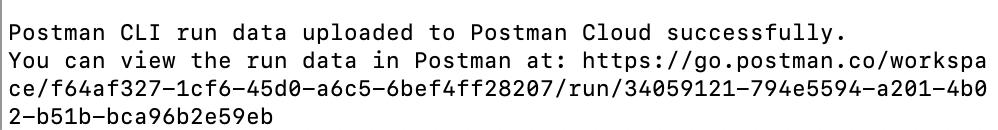
\includegraphics[width=0.8\textwidth]{images/postman_cli_details}
    \caption{Postman CLI Test Results}
    \label{fig:postman-cli-details}
\end{figure}
\end{enumerate}

\subsection{How we test}

In the testing process of the FastAPI Inventory Management System, we adopt a systemic approach for sending HTTP requests with different methods (e.g., GET, POST, PUT, DELETE), headers, body content (in JSON format), and parameters. The testing methodology involves the following steps:

\begin{enumerate}
    \item \textbf{Request Configuration:} We configure Postman to send HTTP requests to the corresponding endpoints for each functionality being tested. We primarily utilized the GET method to retrieve data from the API endpoints related to bookings, categories, devices, users, and pins. This includes setting up appropriate headers, request bodies, and query parameters as necessary.

    \item \textbf{Test Execution:} Upon sending each request, Postman interacts with the server and awaits the response. Once the response is received, Postman triggers a series of predefined tests.

    \item \textbf{Test Result Analysis:} Postman automatically evaluates the response against the predefined tests and generates detailed test reports. We analyze these reports to identify any failed tests or errors encountered during the testing process.

    \item \textbf{Iterative Testing:} Based on the test results and feedback, we iterate on the testing process, updating test scripts, and re-executing tests as necessary to ensure comprehensive testing and validate the functionality’s correctness.
\end{enumerate}

\subsection{What we test}

The entities and their corresponding test areas include:

\begin{itemize}
    \item \textbf{Bookings:} We tested the ability to retrieve existing bookings from the system. Tests include scenarios where bookings are filtered by specific criteria using parameters such as date, user ID, and locker ID.

    \item \textbf{Categories:} Testing focused on ensuring the proper retrieval of available locker categories. Tests verify that categories are returned with their corresponding properties, such as category name and ID.

    \item \textbf{Devices:} Tests aimed to ensure proper retrieval of device information. Tests include essential details such as owner, purchase status, and device-specific information.

    \item \textbf{Users:} Tests targeted at user management functionalities. Tests verify the email address, name, role (user or admin), and ID.

    \item \textbf{Pins:} Generate Pin Functionality in detail. In the testing of the Generate Pin functionality, we focus on evaluating various aspects to ensure the correctness and reliability of the PIN generation process:
    \begin{lstlisting}[language=Java]
    // Test for HTTP status code
pm.test("Status code is 200", function () {
    pm.response.to.have.status(200);
});

// Test that the response contains a "pin" property
pm.test("Response contains a 'pin' property", function () {
    const jsonData = pm.response.json();
    pm.expect(jsonData).to.have.property("pin"); // Check for "pin" property
});

// Test that the "pin" property is an integer
pm.test("'pin' is an integer", function () {
    const jsonData = pm.response.json();
    pm.expect(jsonData.pin).to.be.a("number"); // Ensure "pin" is a number
});

// Test that the "pin" is between 1000 and 9999
pm.test("The 'pin' is a four-digit number between 1000 and 9999 and the generated 'pin' is unique", function () {
    const jsonData = pm.response.json();
    const pin = jsonData.pin;
    pm.expect(pin).to.be.within(1000, 9999); // Check if "pin" is within the four-digit range
});
\end{lstlisting}

    \begin{itemize}
        \item \textbf{HTTP Status Code Test:} We verify that the server responds with a status code of 200, indicating that the request was successful and the PIN generation endpoint is accessible.

        \item \textbf{Presence of “pin” Property Test:} We confirm that the response body contains a "pin" property, which is essential for identifying and retrieving the generated PIN.

        \item \textbf{Data Type of “pin” Property Test:} It's critical to ensure the value associated with the "pin" property is an integer. This guarantees compatibility with further processing steps within the system and adheres to the expected data format.

        \item \textbf{Validity of Generated PIN Test:} We rigorously validate that the generated PIN adheres to the predefined criteria. The PIN should be a four-digit number, falling within the range of 1000 to 9999.
    \end{itemize}
\end{itemize}

If the Postman test execution for the Generate Pin functionality resulted in all four tests passing successfully.
\begin{figure}[h]
    \centering
    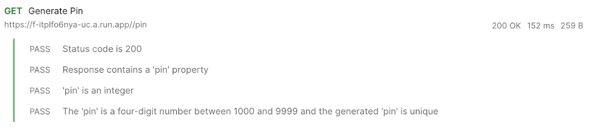
\includegraphics[width=0.8\textwidth]{images/testing1}
    \caption{Generate Pin Functionality Test results}
    \label{fig:testresults-postman}
\end{figure}
This confirms that the API endpoints behaves as intended when generating pins.

\subsection{Evaluation of test results (Automate runs via Postman CLI)}
\begin{figure}[h]
    \centering
    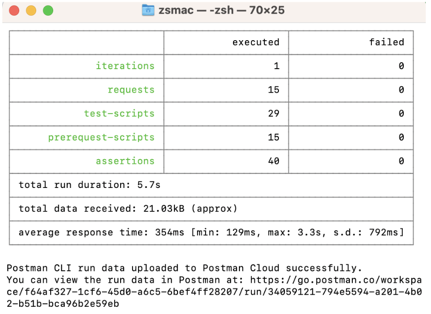
\includegraphics[width=0.8\textwidth]{images/testing2}
    \caption{Test results of Inventory Management System}
    \label{fig:testresults-postman-all}
\end{figure}
We utilise Postman’s command-line interface (CLI) to execute an automated test for our Inventory Management System. The result comprised 29 test scripts designed to verify various functionalities. As show in the picture above, the test run executed all scripts successfully, and the corresponding assertions (verification checks) passed, confirming that the system behaves as intended.